\chapter{Enjeux scientifiques}
\section{Des objectifs définis}
Le projet ORESM a pour objectif d’accompagner la recherche en histoire médiévale en facilitant l’exploitation des sources liées à l’université parisienne au Moyen Âge, au travers un portail web agrégatif. 
\subsection{Alimenter les données de \textit{Studium Parisiense}}
Les données générées par le projet ORESM sont multiples, mais l'accent est mis sur les données concernant la vie des personnes. Puisque celles-ci pourront à terme enrichir la base de données \textit{Studium Parisiense}, il est important que ORESM s'intéresse entre autres aux éléments biographiques des personnes, à leurs mobilités, à leurs activités et à l'ensemble des données prosopographiques. La base de données ORESM sera indépendante de \textit{Studium Parisiense}, mais ces deux bases devront dialoguer pour s'enrichir mutuellement. Cet axe a été pris en compte lors de la manipulation des données issues du projet ORESM.
\subsection{L'élaboration d'un fonds d'archives de l'université de Paris}
Il est question ici de fonds d’archives. Un fonds d'archives désigne un ensemble cohérent de documents produits ou reçus par une personne, une famille, une organisation ou une institution dans le cadre de leurs activités. Ces documents partagent un lien organique du fait de leur origine commune. Dans notre cas nous considérons comme tel tous les documents produits par l’université au Moyen Âge, mais appartiennent également à ce fonds les archives produites par des personnes en faisant partie. Nous intégrons aussi des documents concernant les collèges de l’université et d’autres institutions qui ont eu un lien avec celle-ci. Il est question avec le projet ORESM, de restituer l'épaisseur archivistique d'un tel fonds, à travers des métadonnées riches. Le comité scientifique a également souligné son intérêt, concernant la tradition et le parcours des différentes pièces d'archives entre les nombreuses institutions qui les ont conservées.
\section{État d'avancement}
\subsection{Inventaire EAD}
Dans l'optique de regrouper virtuellement les archives de l'université de Paris, actuellement disséminées, un inventaire\footnote{L'inventaire en terme archivistique est un instrument de recherche, généralement structuré, utiliser pour se retrouver dans un fond d'archives. Il décrit avec des informations plus ou moins précises les éléments qui composent ce fond.} a été réalisé. C'est Arsène Georges qui s'est chargé de réaliser cet inventaire durant son stage en 2021 \footnote{\cite{georges_reunion_2021}}. Cet inventaire est encodé suivant le format XML-EAD\footnote{\href{https://www.loc.gov/ead/}{https://www.loc.gov/ead/}}. Il inclut des descriptions provenant des inventaires des Archives nationales, déjà encodés en EAD, de l'inventaire des archives de la BIS disponible sur Calames également en EAD et les archives conservées à la BIUS, décrites en ligne au format texte, qu'Arsène a lui même encodé en EAD. Le plan de classement utilisé pour réaliser cet inventaire devra être revu par la suite afin d'intégrer les notices issues du travail entrepris pour décrire précisément à la pièce les archives de l'université, jusqu'ici décrites beaucoup plus sommairement. Malgré cela l'inventaire virtuel dans sa forme actuelle est dans sa phase finale puisqu'il est actuellement prévu de le publier sur le site web une fois les derniers réglages effectués. La mise en ligne est prévue avec l'outil \textit{Archives Space}\footnote{\href{https://archivesspace.org/}{https://archivesspace.org/}}.
\begin{figure}[!h]
    \centering
    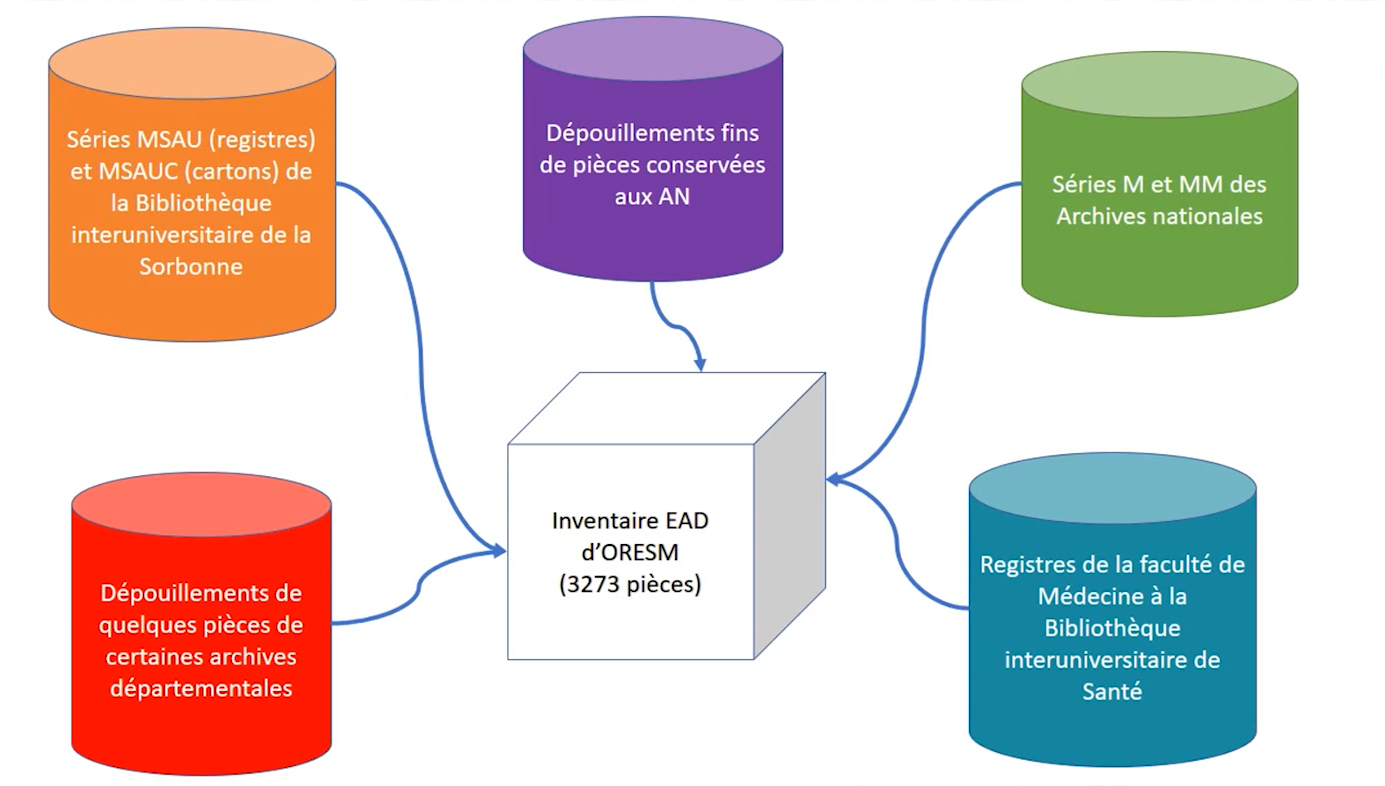
\includegraphics[width=0.8\linewidth]{images/Visualisation inventaire.png}
    \caption{Représentation du regroupement virtuel des notices archivistiques dans un même instrument de recherche.}
    \label{fig:visualisation-inventaire}
\end{figure}
\subsection{Dépouillements d'archives}
Lors de la construction de l'inventaire par Arsène un constat a été fait concernant les notices. Leurs contenus ne répondaient pas aux besoins des enjeux scientifiques du projet, notamment en ce qui concerne les entités nommées. Grâce à un financement du Labex Hastec la BIS a décidé de recruter Louise Gousseau, archiviste, afin de mener une campagne de dépouillements. Cette campagne a permis d'extraire des documents originaux les informations que le conseil scientifique a jugées nécessaires au projet. Le projet ORESM a pour ambition de faire dépouiller l'ensemble du fonds d'archives de l'ancienne université de Paris. Nous reviendrons en détail sur ces dépouillements, puisque les données produites sont au cœur des réalisations de ce stage.
\subsection{Preuve de concept de 2021}
Florence Clavaud a réalisé en 2021, sur une courte période de temps, une preuve de concept visant à démontrer la faisabilité et l'intérêt de la sémantisation des données ORESM dans un graphe de connaissance\footnote{Voir le support utilisé pour présenter cette preuve de concept lors d'une \href{https://oresm.hypotheses.org/files/2022/03/ORESM_JE_26112021_JFMoufflet_FClavaud-3.pdf}{journée d'étude en 2021.}}.  L'idée de cette preuve de concept était de produire ce qui va constituer le coeur du futur portail, à partir de l'ensemble des données disponibles dans les divers formats utilisés (EAD, Excel, référentiel Studium Parisiense). Pour cela il fallait choisir ou définir un modèle unique qui garantisse un haut niveau de granularité et d'exploitabilité, et qui permette par la suite de réutiliser les données. Les technologies sémantiques paraissaient une bonne méthode. Cette preuve de concept a posé les bases du traitement qui sera réalisé sur les données, et présenté dans ce mémoire. Le stage a étendu cette preuve de concept dans sa profondeur et sa portée. Nous reviendrons largement dans les parties suivantes sur celle-ci.